\subsection{Topography relaxation}\label{sec:crameri}
This experiment is performed as in \citet{Crameri2012} using free surface and sticky air (Case 1). The domain is rectangular with $L_x=$ \SI{2800}{\km} and
$L_y=$ \SI{700}{\km} in case of free surface and $L_y=$ \SI{800}{\km} in case of sticky air ($h_{st}=$ \SI{100}{\km}). The grid is composed by $256\times64$
elements for the free surface $560\times320$ elements for the sticky air. For both cases, there is a mantle of 600 km thickness with $\eta_m=$ \SI{e21}{\pascal\s}
overlain by a highly viscous cosine-shaped lithosphere with thickness between 93 and 107 km and $\eta_l=$ \SI{e23}{\pascal\s}. Both mediums have $\rho=$
\SI{3300}{\kg\per\cubic\metre}. In case of sticky air experiment, the air has $\rho_a=$ \SI{0}{\kg\per\cubic\metre} and $\eta_a=$ \SI{e18}{\pascal\s}. The
gravity acceleration is set to $g_y=$ \SI{-10}{\metre\per\square\s}. Velocity boundary conditions are set to no slip at the bottom and free slip at the sides
of the domain. In case of sticky air, velocities on top are set to free slip conditions.
\begin{wrapfigure}{l}{12cm}
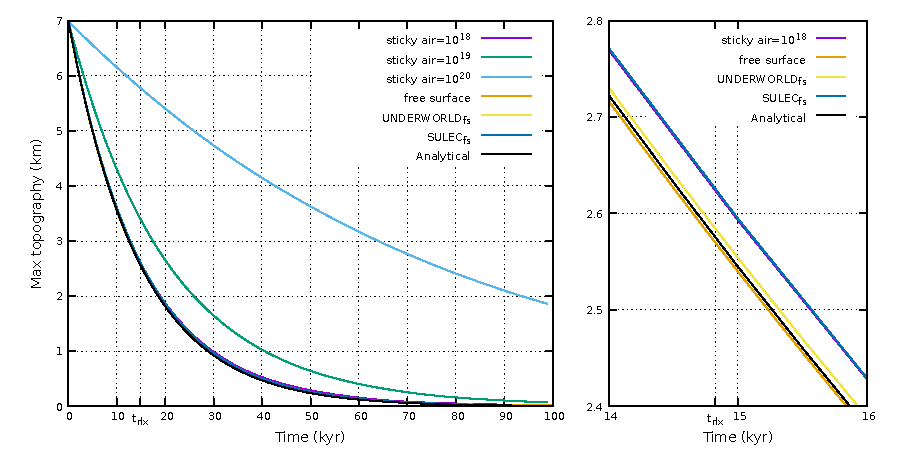
\includegraphics[width=12cm]{./Figures/Crameri.pdf}
\caption{Maximum topography as function of time for the Crameri benchmark (coloured lines) in comparison with the analytical solution (black line) and results
shown by \citet{Crameri2012} with UNDERWORLD (yellow line) and SULEC (blue line).}
\label{fig:crameri}
\end{wrapfigure}
The maximum topography as function of time ($h(t)$) can be analytically derived in according to
\begin{eqnarray}
h(t)=h_0 \exp(\gamma t)\nonumber
\end{eqnarray}

where $h_0=7$ km is the initial topography, $\gamma=\num{-0.2139e-11}$ is the characteristic relaxation rate and $t$ is the time (black line in Fig.
\ref{fig:crameri}). Maximum topography at the characteristic relaxation time $t_{rlx}=$ \SI{14.825}{\kilo\year} can be found to be $h_{rlx}=$ \SI{2576}{\m}.
The results show that a viscosity of the air of \SI{e18}{\pascal\s} is needed in case of $h_{st}=$ \SI{100}{\km} to correctly describe the topography relaxation
for this problem, as pointed out by \citet{Crameri2012} (purple line in Fig. \ref{fig:crameri}). The case with a true free surface well follows the analytical
solution (orange line in Fig. \ref{fig:crameri}). In particular, at the relaxation time in case of the true free surface predicts a maximum topography of
\SI{2570}{\m}, with an error of \SI{6}{\m} with respect to the analytical solution. Results are also compared with results obtained with a free surface in
UNDERWORLD $256\times64$ elements) and SULEC ($401\times201$ elements) (with courtesy from \citealp{Crameri2012}). All data can be 
found at \url{https://github.com/aleregorda/Benchmarks/tree/main/Surface_processes/Topography_relaxation}.